\documentclass[tikz,border=2pt]{standalone}
\usepackage{pgfplots}
\pgfplotsset{compat=newest}
\begin{document}


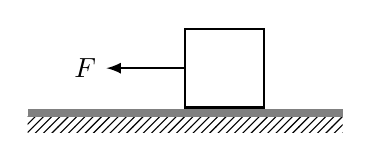
\begin{tikzpicture}
\newcommand{\ground}[2][]{
\begin{scope}[#1]
\usetikzlibrary{patterns,calc}
\def\groundlen{#2}
\fill[pattern = north east lines] (-#2,0) rectangle (#2,0.2);
\fill[color=black!50] (-#2,0.2) rectangle (#2,0.3);
\end{scope}}

\ground[yshift=-9]{2cm}

\draw[thick]  (0,0) rectangle (1,1);
\draw[thick,-latex] (0,0.5) -- (-1,0.5) node[left] {$F$};


\end{tikzpicture}


\end{document}